\documentclass[11pt,a4paper]{article}
\usepackage[T1]{fontenc}
\usepackage[utf8]{inputenc}
\usepackage{lmodern}
\usepackage[margin=2.5cm]{geometry}
\usepackage{amsmath,amssymb}
\usepackage{booktabs}
\usepackage{graphicx}
\usepackage[hidelinks]{hyperref}
\hypersetup{pdfauthor={Gianni Pilotti},pdftitle={Pricing and Risk of Structured Products: Greeks, Monte Carlo and Hedging},pdfcreator={},pdfproducer={}}
\setlength{\parindent}{0pt}
\setlength{\parskip}{6pt}

\title{Pricing and Risk of Structured Products:\\Greeks, Monte Carlo and Hedging}
\author{Gianni Pilotti}
\date{}

\begin{document}
\maketitle

\section{The Core Idea}
A structured product is a bond plus options, and its risk is the risk of those options. A Phoenix autocall, for example, pays coupons, can be redeemed early, and loses capital if the underlying ends low. It has no closed-form price. A risk manager still needs its price, its sensitivities, and the effect of hedging it.

The repository (\texttt{structrisk}) does four things for this.
\begin{itemize}
\item \textbf{Closed-form Greeks} of a vanilla option, from first order (delta, vega) to third order (speed, zomma, color).
\item \textbf{Monte Carlo pricing} of a Phoenix autocall and of other notes, with confidence intervals. Sensitivities come from bump-and-revalue with common random numbers.
\item \textbf{Portfolio risk:} Greeks added across positions, in euros, with a spot-by-volatility stress grid.
\item \textbf{Hedging simulation:} the replication error of a delta-hedged option, with and without costs.
\end{itemize}

\section{Method}
\subsection{Black-Scholes-Merton Greeks}
With dividend yield $q$, $d_1=\dfrac{\ln(S/K)+(r-q+\tfrac12\sigma^2)T}{\sigma\sqrt T}$ and $d_2=d_1-\sigma\sqrt T$, the call Greeks are:

\begin{center}
\begin{tabular}{@{}lll@{}}
\toprule
Greek & Formula & Note \\
\midrule
Delta & $e^{-qT}N(d_1)$ & per unit of spot \\[2pt]
Gamma & $\dfrac{e^{-qT}\varphi(d_1)}{S\sigma\sqrt T}$ & same for call and put \\[6pt]
Vega & $S e^{-qT}\varphi(d_1)\sqrt T$ & per 1.00 of vol \\[2pt]
Vanna & $-e^{-qT}\varphi(d_1)\,d_2/\sigma$ & $\partial\Delta/\partial\sigma$ \\[2pt]
Volga & $\text{Vega}\cdot d_1d_2/\sigma$ & $\partial\text{Vega}/\partial\sigma$ \\
\bottomrule
\end{tabular}
\end{center}
Charm, speed, zomma, color and veta are also implemented in closed form.

\subsection{Phoenix autocall by Monte Carlo}
Spot paths follow geometric Brownian motion with drift $r-q$, simulated at the observation dates with antithetic variates. At each date $t_j$ with performance $P_j=S_{t_j}/S_0$:
\begin{itemize}
\item \textbf{Early redemption:} if $P_j\ge$ the autocall barrier (and $j$ is not the last date), the notional is repaid at $t_j$.
\item \textbf{Coupon with memory:} if $P_j\ge$ the coupon barrier, the holder receives the coupon times the number of periods since the last payment. Missed coupons are paid when the barrier is next met.
\item \textbf{At maturity:} if the product was never called, the notional is repaid when $P_n\ge$ the protection barrier, and $N\times P_n$ otherwise.
\end{itemize}
The price is the mean of discounted cash flows, $\sum_j c_j e^{-rt_j}+R\,e^{-r\tau}$, with a 95\% interval $\pm1.96\,s/\sqrt{n}$. Greeks are central differences of the price with the same seed in every bump (common random numbers), so the payoff discontinuities do not turn into noise.

\subsection{Portfolio aggregation}
For positions with quantity $q_i$, multiplier $m_i$ and spot $S$:
\begin{align*}
\text{Delta-equivalent exposure}&=\sum_i q_im_i\,\Delta_i\,S,\\
\text{Gamma P\&L for }+1\%&=\tfrac12\sum_i q_im_i\,\Gamma_i\,(0.01\,S)^2,\\
\text{Vega P\&L per vol point}&=0.01\sum_i q_im_i\,\mathcal{V}_i .
\end{align*}
The stress grid uses, for each position, $\Delta\,dS+\tfrac12\Gamma\,dS^2+\mathcal{V}\,d\sigma+\text{Vanna}\;dS\,d\sigma$, with $dS=\text{shock}\times S$.

\subsection{Delta-hedging simulation}
A call is sold for its Black-Scholes premium. At each of $n$ dates, the position holds the model delta in shares, pays a cost of $c$ bp on the traded notional, and earns the dividend on the shares. At expiry, the replication error is the portfolio value minus the option payoff.

\section{Results}
\textbf{Greeks.} ATM call, 1 year, $r=3\%$, $q=2\%$, $\sigma=22\%$: delta 0.5506, gamma 0.01756, vega 38.635, theta $-0.0124$ per day. ATM gamma at 1 month (0.08 year) is 0.06395 against 0.01203 at 2 years, a ratio of 5.32.

\textbf{Phoenix autocall.} Spot 100, volatility 25\%, $r=3\%$, $q=2\%$, observations every six months for two years, 4\% coupon per period, barriers 100\% (call), 70\% (coupon) and 60\% (capital), 200,000 paths.

\begin{center}
\begin{tabular}{@{}lc@{}}
\toprule
Quantity & Value \\
\midrule
Price (\% of notional) & 100.71 (95\% interval 100.64 to 100.77) \\
Called at 0.5 year & 47.59\% \\
Called at 1.0 year & 11.93\% \\
Called at 1.5 years & 6.10\% \\
Never called & 34.38\% \\
Capital loss, given never called & 22.71\% \\
\bottomrule
\end{tabular}
\end{center}
Raising the call barrier from 95\% to 105\% moves the price from 100.51 to 101.05. Recomputed with the repository function (same seed), the price has delta 0.173 per unit of spot and vega $-52.7$ per 1.00 of volatility, so the holder is short volatility.

\begin{figure}[h]
\centering
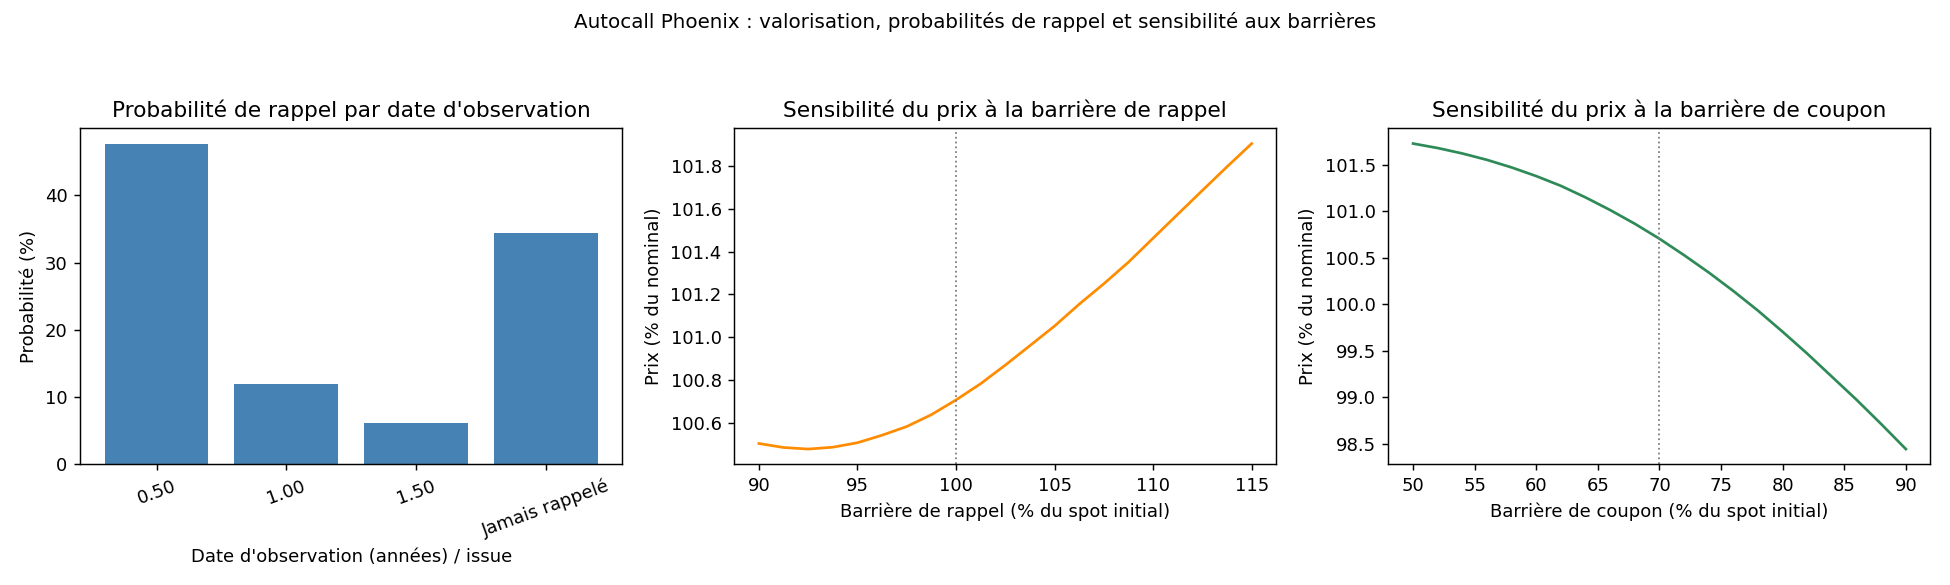
\includegraphics[width=0.98\textwidth]{../docs/img/03_autocall_pricing.png}
\caption{Phoenix autocall: probability of each outcome and price against the call and coupon barriers (labels in French).}
\end{figure}

\textbf{Portfolio.} Long 1,000 calls (strike 105) and short 600 puts (strike 95), both 1 year, plus 50 capital-protected notes and 30 capped bonus certificates, on one underlying (spot 100, volatility 22\%). Delta-equivalent exposure is EUR 66,931. A $+1\%$ move in spot adds EUR 3.92 through gamma, and one volatility point adds EUR 235.88. The spot-by-volatility grid (spot $\pm20\%$, volatility $\pm10$ points) goes from EUR $-12{,}827$ to $+18{,}663$.

\textbf{Delta hedging.} Short call, spot 100, strike 100, 6 months, volatility 25\%, 40,000 paths. The error is in units of the option price:

\begin{center}
\begin{tabular}{@{}rccc@{}}
\toprule
Rehedges & Std, no cost & Mean, 10 bp cost & Std, 10 bp cost \\
\midrule
1 & 5.3962 & $-0.1120$ & 5.3962 \\
4 & 2.8543 & $-0.1235$ & 2.8641 \\
12 & 1.6970 & $-0.1660$ & 1.7075 \\
52 & 0.8388 & $-0.2812$ & 0.8523 \\
252 & 0.3894 & $-0.5570$ & 0.4407 \\
\bottomrule
\end{tabular}
\end{center}
More rehedging narrows the error but costs more. The mean cost grows from 0.11 to 0.56 between 1 and 252 rehedges.

\section{Worked Example}
\textbf{Greeks by hand} for the ATM call above ($S=K=100$, $T=1$, $r=3\%$, $q=2\%$, $\sigma=22\%$):
\begin{align*}
d_1&=\frac{(0.03-0.02+0.5\times0.22^2)\times1}{0.22}=\frac{0.0342}{0.22}=0.1555,\\
N(d_1)&=0.5618,\quad \varphi(d_1)=0.3942,\quad e^{-qT}=0.9802,\\
\Delta&=0.9802\times0.5618=0.5506,\\
\Gamma&=\frac{0.9802\times0.3942}{100\times0.22}=0.01756,\\
\mathcal{V}&=100\times0.9802\times0.3942=38.63 .
\end{align*}

\textbf{One Phoenix path} (illustrative): performances at the four dates are 65\%, 80\%, 72\%, 58\%, with notional 100. The coupon is $4\%\times100=4$ per period.
\begin{itemize}
\item $t=0.5$: 65\% is below the 70\% coupon barrier, no coupon (one period is owed).
\item $t=1.0$: 80\% is above 70\%, so the coupon is paid for two periods: $4\times2=8$.
\item $t=1.5$: 72\% is above 70\%, coupon $4$.
\item $t=2.0$: 58\% is below 70\%, no coupon. It is also below the 60\% protection barrier, so redemption is $100\times0.58=58$.
\end{itemize}
Present value at $r=3\%$: $8e^{-0.03}+4e^{-0.045}+58e^{-0.06}=7.764+3.824+54.622=66.21$. The same path with a performance of 105\% at the first date pays $4$ and redeems $100$ at $t=0.5$.

\section{Limits}
\begin{itemize}
\item \textbf{Constant volatility:} no stochastic volatility or jumps. The volatility surface in the examples is a synthetic parametrisation, not market data.
\item \textbf{No credit risk:} issuer risk is not in the structured product prices, although it is a large part of the risk of a note.
\item \textbf{Barrier monitoring:} barriers are checked on the simulation grid, not continuously.
\item \textbf{Portfolio example:} the bonus certificate is given a zero vega in the portfolio, so the EUR 235.88 per vol point leaves out its volatility sensitivity. The stress grid is a second-order expansion with a vanna term, not a full revaluation.
\item \textbf{Hedging scaling:} the error does not fall exactly as $1/\sqrt n$. From 1 to 252 rehedges, the rule gives $5.3962/\sqrt{252}=0.340$ and the simulation gives 0.389. These are model outputs, not recommendations.
\end{itemize}

\end{document}
